\scanpage{1}
% not manuscript: couverture institutionnelle de l'Université de Montpellier et de l'IMAG.

\scanpage{2}
\unsure{Pages|Page} 650--787 + table of contents

\uline{N.B.} Page 650 appears twice (numbering error)

\margin{1}

% Pied de page imprimé de l'archive.
\begin{center}
\small
1\\
\texttt{https://grothendieck.umontpellier.fr}\\
Université de Montpellier, UMR CNRS 5149, Case courrier 051, Place Eugène Bataillon\\
34095 Montpellier cedex 5 - France
\end{center}

\scanpage{3}
50. Schematic envelopes of discrete groups: metabelian case \hfill 650

1°) Unipotent sections \hfill same

2°) Attempt at a \unsure{characterization} of quasi-unipotent sections \hfill $652'$

3°) Group scheme associated with certain extensions of discrete groups (abelian kernel) \hfill $\unsure{655'}$

4°) Schematic envelope of a metabelian group \hfill $658'$

5°) Universal characterizatio\textsuperscript{n} of the schematic envelope \hfill $\unsure{662'}$

51. Example: the Fermat tower. \hfill 664

1°) The groups $\mathfrak S=\mathrm{Sl}(2,\mathbb Z)/[\Pi_0,\Pi_0]$, and $\underline{\mathfrak S}$ \hfill same

2°) $\unsure{\underline Z|Z}_{\rho,\sigma}$: provisional version \hfill $665'$

3°) The groups $\Phi_N^*$ and variants \hfill 673

4°) The sequence
\diagram{\begin{tikzcd}[column sep=small]
1 \arrow[r] & \underline N^{0+}_{\rho,\sigma} \arrow[r] & \underline N_{\rho,\sigma} \arrow[r] & \Phi_{12}^{*} \arrow[r] & 1
\end{tikzcd}},
and relations with $\mathrm{Sl}(2,\mathbb Z/12\mathbb Z)$ \hfill 677

5°) $\underline M_{\rho,\sigma}$, $\underline M^{\unsure{\natural|\sharp}}_{\rho,\sigma}$ via $N_{\rho,\sigma}$ \hfill 682

6°) \deleted{$\unsure{\underline Z_{\rho,\sigma}}$} \unsure{sequences}
\diagram{\begin{tikzcd}[column sep=small]
1 \arrow[r] & \mathbb G_a \arrow[r] & \underline Z_{\rho,\sigma} \arrow[r] & \widehat\Phi_{12} \arrow[r] & 1
\end{tikzcd}},
and
\diagram{\begin{tikzcd}[column sep=small]
1 \arrow[r] & \underline{\mathfrak S}^{+} \arrow[r] & \underline G_{\rho,\sigma} \arrow[r] & \widehat\Phi_{12} \arrow[r] & 1
\end{tikzcd}}
\hfill 684

7°) $\underline N_\rho$, $\underline N_\rho^{\unsure{\natural|\sharp}}$ and so on \hfill 686

8°) $\underline N_\sigma$, $\underline N_\sigma^{\unsure{\natural|\sharp}}$ and so on \hfill 689

9°) Return to $\underline M_{\rho,\sigma}$, $\underline M_{\rho,\sigma}^{\unsure{\natural|\sharp}}$ and so on \hfill 690

10°) $\underline M_{\rho,\sigma}\unsure{(0)|[0]}$, $\underline M_{\rho,\sigma}\unsure{[\tfrac12]|(\tfrac12)}$, $\underline M_{\rho,\sigma}(-\bar j)$ and so on \hfill $691'$

11°) The homomorphism $M\longrightarrow M_{\rho,\sigma}=\underline M_{\rho,\sigma}(\widehat{\mathbb Z})^{\wedge}$, and relations with the tower of Fermat curves: statement of the problem. \hfill 695

12°) Splittings of the extension $G_{\rho,\sigma}/\mu_G$ of $\widehat{\mathbb Z}^{*}\times\mathfrak S_3$ by $\widehat M$. \hfill 700

13°) \deleted{\unsure{Digression on}}\inserted{Characterization of} the Fermat tower; \deleted{and} \deleted{\unsure{conjectures}}\inserted{relations} of compatibility, with $M\longrightarrow G_{\rho,\sigma}$ \hfill \deleted{\unsure{703}}\inserted{707}

14°) Relation with generalized Jacobians \hfill $\unsure{720'}$

15°) Interpretation of $\unsure{\Gamma_{\mathbb Q}}\longrightarrow N_\sigma^{\unsure{\natural|\sharp}}\simeq\unsure{\widehat{\mathbb Z}}^{*}\mathbin{.}\widehat{\mathbb Z}$, and digression on \unsure{Kummer} extensions \hfill $725'$

16°) Reflections on Fermat's theorem \hfill 733

\margin{2}

% Pied de page imprimé de l'archive.
\begin{center}
\small
2\\
\texttt{https://grothendieck.umontpellier.fr}\\
Université de Montpellier, UMR CNRS 5149, Case courrier 051, Place Eugène Bataillon\\
34095 Montpellier cedex 5 - France
\end{center}

\scanpage{4}
52. \deleted{Schematic envelopes of L-groups and $\Pi L$-groups.}\inserted{Lie approximations of Galois-Teichmüller systems.}

1°) Notion of L- and $\Pi L$-group: discrete case \hfill 737

2°) Profinite case \hfill 744

3°) \deleted{\unsure{Discretification}, and \unsure{admissible homomorphisms},}\inserted{Lie approximations of systems} of Galois-Teichmüller \hfill 748

4°) Lie approximation induced by a ``geometric'' Lie approximation \hfill 758

\uline{53}. The special Teichmüller group $\unsure{S\mathcal T}_{1,1}\simeq\mathrm{Gl}(2,\mathbb Z)^{\sim}$, and the group $SN_{1,1}$ \hfill 760

1°) Differential action and special Teichmüller group (provisional statement) \hfill same

2°) The groups $\mathrm{Gl}(2,\mathbb R)^{\pm1\,\sim}$, $\mathrm{Sl}(2,\mathbb R)^{\sim}$ \hfill $761'$

3°) The group $\mathrm{Gl}(2,\mathbb Z)^{\sim}$ \hfill 763

4°) The isomorphism $\mathrm{Gl}(2,\mathbb Z)^{\sim}\simeq\unsure{S\mathcal T}_{1,1}$ \hfill $\unsure{766'|765'}$

5°) Digression on coverings of germs of spaces, and relations between topological germs and differentiable germs of surfaces \hfill $768'$

6°)

% Right-hand page of the spread: blank.

\margin{3}

% Pied de page imprimé de l'archive.
\begin{center}
\small
3\\
\texttt{https://grothendieck.umontpellier.fr}\\
Université de Montpellier, UMR CNRS 5149, Case courrier 051, Place Eugène Bataillon\\
34095 Montpellier cedex 5 - France
\end{center}

\scanpage{5}
\mspage{650\ \textcircled{bis}}

50. \uline{Schematic envelopes of discrete groups.}

\deleted{\unsure{2}}(\uline{Metabelian case})

1.\deleted{\unsure{g}} Let $G$ be a group scheme locally of finite presentation
over a base scheme $S$ (the case \unsure{important} for us will be
$S=\operatorname{Spec}(\mathbb Z)$). A section $g$ of $G$ over $S$ is said to be
\uline{unipotent} if on every geometric fiber,
\deleted{\unsure{of}} $G_{\bar s}$, the element
$g_{\bar s}\in G_{\bar s}(\unsure{\bar k|k^a})$
$(k=k(\bar s))$ is unipotent, i.e. if there exists a group homomorphism
\margin{\uline{Unipotent \unsure{sections}}}
\[
(1)\qquad \mathbb G_{ak}\xrightarrow{\varphi_{\bar s}}G_k
\qquad k=k(\bar s)
\]
such that
\[
(2)\qquad g_{\bar s}=\varphi_{\bar s}(1)
\]

We say that $g$ is quasi-unipotent if for every $\bar s$, there exists
$n\in\mathbb N^*$ such that $g_{\bar s}^{n}$ is unipotent.
If the characteristic of $\bar s$ is $p>0$, then this also \uline{means} that
$g_{\bar s}$ is of \uline{finite order}. We see that if $S$ is
quasi-compact, then $g$ is quasi-unipotent iff
$\exists n\in\mathbb N^*$ such that $g^n$ is unipotent.

\deleted{\uline{Theorem} -- Let $G$ \inserted{of groups}
be locally of finite presentation over quasi-compact $S$,
$\unsure{g|G}$ \unsure{if|which} is \unsure{unipotent|unipotent}, \unsure{for a}}

\deleted{\unsure{?}} For $g$ to be unipotent, it \uline{suffices} that there exist a homomorphism
\[
(3)\qquad \varphi:\mathbb G_a\longrightarrow G
\]
\margin{4}

% Pied de page imprimé de l'archive.
\begin{center}
\small
4\\
\texttt{https://grothendieck.umontpellier.fr}\\
Université de Montpellier, UMR CNRS 5149, Case courrier 051, Place Eugène Bataillon\\
34095 Montpellier cedex 5 - France
\end{center}

\scanpage{6}

such that we have
\[
(4)\qquad \varphi(1)=g.
\]

I wonder whether this is also necessary, in ``good'' cases. Let us first take the
case where $S=\operatorname{Spec}K$. In characteristic $0$, we have a uniqueness
result for $\varphi$, which allows us to apply descent theory
(valid over any base \uline{in characteristic $0$}): if after an extension
$S'\longrightarrow S$ faithfully flat \unsure{quasi-compact}, there exists $\varphi'$ having
the desired properties, then $\varphi$ exists
(over $S$ \unsure{itself|=}).
So over a \uline{field} of characteristic $0$ it is OK. In characteristic $p>0$ the difficulty
comes from the fact that there are group homomorphisms
\inserted{$\mathbb G_a\longrightarrow\mathbb G_a:$}
(such as $x\mapsto x^p-x$) which are \deleted{zero} nontrivial, and which are
trivial on $1$. We shall get around this \inserted{perhaps} by applying
\unsure{descent} with $\varphi$ which are \uline{monomorphisms}.
\deleted{Every} \inserted{\unsure{This raises the question:|This leads to the question:}}
Is a subgroup of $G$ \unsure{isomorphic} to $\mathbb G_a$ known when
we know an everywhere nontrivial section? Is this at least true over a
\uline{field} as base?

I do not feel like launching into these questions (certainly interesting!),
and prefer
\margin{5}

% Pied de page imprimé de l'archive.
\begin{center}
\small
5\\
\texttt{https://grothendieck.umontpellier.fr}\\
Université de Montpellier, UMR CNRS 5149, Case courrier 051, Place Eugène Bataillon\\
34095 Montpellier cedex 5 - France
\end{center}

\scanpage{7}
\mspage{651}

to limit myself to a case closer to the one I am after, $S=\operatorname{Spec}\mathbb Z$,
assuming $S$ noetherian integral, \deleted{\unsure{of characteristic}} with generic point $\eta$
of characteristic $0$. This already implies, by the result over a field of characteristic $0$,
that there exists a nonempty open $U$
\[
(5)\qquad
\underset{\substack{\text{open}\\\text{nonempty}}}{U\subset S}
\quad\text{and}\quad
\deleted{g_U}\;\varphi_U:\mathbb G_a\vert U\longrightarrow G\vert U
\]
such that we have (4) \uline{on} $U$ -- and (for $U$ chosen) this $\varphi_U$
is unique. By uniqueness, we thus see that there is a largest open
\inserted{$\unsure{\mathcal U|U}$} over which we can give such a
$\unsure{\varphi|\psi}_{\unsure{\mathcal U|U}}$,
and the question comes down to seeing whether we necessarily have $\unsure{\mathcal U|U}=S$.

If we had $U\ne S$, localizing if necessary at a maximal point of $\unsure{S\setminus\mathcal U|S\setminus U}$,
we \deleted{\unsure{can}} reduce to examining the case where $S$ is local,
with closed point $s$ -- and to \inserted{\unsure{trying to|a little of}} prove
that in this case, we can extend $\varphi_U$ over all of $S$
(whence a contradiction\ldots). In the case which interests us, $S$ is
\uline{regular} of dimension $1$, so by localizing we find a \uline{trait}.
I shall confine myself to this case, \unsure{crucial}
\margin{6}

% Pied de page imprimé de l'archive.
\begin{center}
\small
6\\
\texttt{https://grothendieck.umontpellier.fr}\\
Université de Montpellier, UMR CNRS 5149, Case courrier 051, Place Eugène Bataillon\\
34095 Montpellier cedex 5 - France
\end{center}

\scanpage{8}

\unsure{,|.} probably if we want to elucidate the general case, and which suffices for
my purpose.

Let $\eta$ be the generic point of $S$, $s$ its closed point. Consider the
subgroup $L_\eta=\varphi_\eta(\mathbb G_{a\eta})\subset G_\eta$,
let $L$ be its schematic closure in $G$. which is a reduced subgroup scheme
of $G$. Let \deleted{\illegible{1} $L$}
$L^0=L\setminus
\bigl(\underset{\substack{\text{components}\\\text{of }L_s\text{ non-}\\\text{identity}}}{\bigcup L_{s,i}}\bigr)$
be its identity component. We have \unsure{won} if we \unsure{prove} that
$L^0\simeq\mathbb G_{aS}$. In fact, we are not
\unsure{even|=} sure that
$(L_s^0$ \deleted{\unsure{is}} $(=(L_s)^0)$ is reduced!
But for $\varphi:\mathbb G_{aS}\longrightarrow G$
\deleted{such that} extending $\varphi_\eta$ to exist, it is probably not necessary
that we have $L^0\simeq\mathbb G_a$ -- for it is possible that
$\varphi$ is not a monomorphism, i.e. that $\varphi_s$ is not a monomorphism --
it could \unsure{even|=} be the trivial homomorphism
(if $g_s=1$)! But even if $g_s\ne1$, it is not clear that
$\varphi_s$ is a monomorphism.

Let us take the example where
\[
(6)\qquad G=\underline{\operatorname{Aut}}_{\mathcal O_S}(M)
\simeq\operatorname{Gl}(n)_S
\]
$M$ a \deleted{\unsure{a}} free module of rank $n$ over $S$,
then we shall have (since $\eta$ of characteristic $0$)
\[
(7)\qquad
\varphi_\eta(\lambda)=\sum\frac{X^{i}_{\unsure{\eta}}}{i!}\lambda^i
\]
where
\[
\unsure{X_\eta|X}\in\operatorname{End}_{\unsure{K}}(M_K)
\qquad K=k(\eta)
\]
\margin{7}

% Pied de page imprimé de l'archive.
\begin{center}
\small
7\\
\texttt{https://grothendieck.umontpellier.fr}\\
Université de Montpellier, UMR CNRS 5149, Case courrier 051, Place Eugène Bataillon\\
34095 Montpellier cedex 5 - France
\end{center}

\scanpage{9}
\mspage{652}

is a \uline{nilpotent} endomorphism of $M_K$.
thus an element \deleted{of $\operatorname{End}(M)\otimes_A K$}
\[
(8)\qquad X\in\operatorname{End}_A(M)\otimes_A K,\qquad X^n=0.
\]
($A$ the affine ring of $S$, which is a \deleted{\illegible{1}} gauge)
We shall have by hypothesis
\[
g_\eta=\varphi_\eta(1)=\sum\frac{X^i}{i!}\in
\diagram{\begin{tikzcd}[ampersand replacement=\&,row sep=1.6em]
\operatorname{Aut}(M)\arrow[d,phantom,"\cap" description]\\
\operatorname{Aut}(M_K)
\end{tikzcd}}
\]
i.e.
\[
(9)\qquad \sum\frac{X^i}{i!},\quad
\sum(-1)^i\frac{X^i}{i!}\in\operatorname{End}_A(M)
\]
and the question whether $\varphi_\eta$ comes from a homomorphism of groups
$\mathbb G_a\longrightarrow G$ comes down to that of knowing whether
\[
(10)\qquad \frac{X^i}{i!}\in\operatorname{End}_A(M)
\qquad\forall\,\unsure{(1\le i\le n-1)|1\le i\le n-1}
\]
\margin{(for $i=0$ and $\unsure{i\ge n|i=n}$ this is trivial)}

For $n=2$ this is trivial, For $n=3$ \uline{\unsure{ditto|ditto}}
(in (9) there is a single term with a denominator).
\[
\deleted{\varphi_\eta(\lambda)=1+X\lambda+\frac{X^2}{2}\lambda^2
\qquad\left\{\begin{array}{l}X\in M_3(K)\\X^3=0\end{array}\right.}
\]
the first \unsure{doubtful} case is $n=4$
\deleted{and the question is to know whether}
\[
\varphi_\eta(\lambda)=1+X\lambda+\frac{X^2}{2}\lambda^2+
\frac{X^3}{6}\lambda^3
\qquad\begin{array}{l}X\in M_4(K)\\X^4=0\end{array}
\]
we have by hypothesis $\varphi_\eta(1)$ and $\varphi_\eta(-1)$ in $M_4(A)$,
i.e.
\[
(11)\qquad \frac{X^2}{2}\mathbin{\pm}\frac{X^3}{6}\in M_4(A)
\]
we wonder whether it follows that
\[
(12)\qquad \frac{X^2}{2},\frac{X^3}{6}\in M_4(A)\qquad ?
\]
If $2$ invertible in $A$ this is clear, for we deduce from (11) that $X^2\in M_4(A)$
hence $\dfrac{X^2}{2}\in M_4(A)$, hence also $X^3/6\in M_4(A)$, OK.
Thus the difficulty
\margin{8}

% Pied de page imprimé de l'archive.
\begin{center}
\small
8\\
\texttt{https://grothendieck.umontpellier.fr}\\
Université de Montpellier, UMR CNRS 5149, Case courrier 051, Place Eugène Bataillon\\
34095 Montpellier cedex 5 - France
\end{center}

\scanpage{10}
arises here in residual characteristic 2. \deleted{\unsure{Let}} Suppose \deleted{\unsure{$\pi$}} \inserted{for simplicity that 2 is} a \unsure{uniformizer} $\unsure{\pi}$ of $A$, we shall have, if $X\notin M_4(A)$
\[
X=\frac{1}{\unsure{\deleted{\pi}\inserted{2}}^{\nu}}X_0
\quad\text{with}\quad
\begin{gathered}
X_0\in M_4(A)\ \deleted{\unsure{\pi M_4}}\\
X_0\notin \unsure{\deleted{\pi}\inserted{2}}M_4(A)
\end{gathered}
\]
hence \deleted{\unsure{and the}} the datum of $X$ is equivalent to that of
\[
X_0\unsure{=|\in}\deleted{\illegible{1}}(a_{ij})_{1\leq i,j\leq4},\quad
\deleted{\unsure{\in M_4(A)|\in A}}\quad\text{the }a_{ij}\in A\text{ not all}
\]
divisible by 2, with \deleted{$\unsure{X_0^4}$}.
\[
(11\,\text{bis})\qquad X_0^4=0,\qquad
\frac12\frac{X_0^2}{2^{2\nu}}\pm\frac16\frac{X_0^3}{2^{3\nu}}\in M_4(A)
\]
--- and the question is whether it follows that we \unsure{have|have}
\[
(12\,\text{bis})\qquad
\frac12\frac{X_0^2}{2^{2\nu}},\frac12\frac{X_0^3}{2^{3\nu}}\in M_4(A)\qquad ?
\]

Of\deleted{\illegible{1}} course, the \deleted{\unsure{q}} answer is \unsure{trivially|totally} yes, if $X_0^3=0$ \inserted{i.e. $X^3=0$} --- so we are interested in the case where $X_0^3\ne0$, i.e. \deleted{$\unsure{X_{0\eta}}$} $g_\eta$ is ``principal unipotent.

\margin{\uline{Attempt at a characterization of quasi-\deleted{\illegible{1}}unipotent sections}}
2.\quad To get to the bottom of it, one would need a counterexample in the preceding context (with a nilpotent matrix of order 4) --- or a theorem ! But for my purpose, it seems that it is not essential to have a solution of this problem.

On the other hand, I shall try the

\uline{Theorem} (!) Let $G$ be a group scheme \inserted{(separated)} locally of finite presentation over a scheme $S$\deleted{\illegible{1}} which is quasi-compact, and let $g$ be a section of $G$. For $g$ to be quasi-unipotent, it
\margin{9}

% Pied de page imprimé de l'archive.
\begin{center}
\small
9\\
\texttt{https://grothendieck.umontpellier.fr}\\
Université de Montpellier, UMR CNRS 5149, Case courrier 051, Place Eugène Bataillon\\
34095 Montpellier cedex 5 - France
\end{center}

\scanpage{11}
\mspage{653}
\margin{\figure{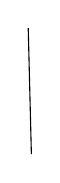
\begin{tikzpicture}[x=1cm,y=1cm]\draw (0,0)--(-0.04,1.6);\end{tikzpicture}}}
is necessary and sufficient that there exist an integer $n>0$, and a homomorphism of group schemes $\varphi:\mathbb G_a\longrightarrow G$, such that we have
\[
(13)\qquad \varphi(1)=g^n.
\]

Sufficiency being trivial, it is a matter of examining necessity. For simplicity, we shall again suppose $S$ noetherian and integral --- once $S$ is assumed noetherian, I think that the reduction to the integral case should be done by easy dévissages, which I do not feel like doing, for lack of essential need ! I shall therefore examine the case $S$ noetherian integral, generic point $\eta$

a) Characteristic \unsure{of} $\eta$ is $>0$. Then \deleted{$\unsure{g_\eta}$} the hypothesis on $g_\eta$ is that $g_\eta$ is of finite order --- hence $\exists n>0$ such that $g_\eta^n=1$, hence $g^n=1$. We shall take in (13) this $n$, and $\varphi$ the trivial homomorphism.

b) Case where $\eta$ of characteristic zero. Let $\varphi$
\[
(14)\qquad \varphi_{1\eta}:\mathbb G_{a\eta}\longrightarrow G_\eta
\]
be defined by the condition
\[
g_\eta=\varphi_{1\eta}(1)
\]
let $U_1$ be its ``open set of definition'' in $S$.

Let
\[
\varphi_{n\eta}(\lambda)=\lambda^n=\varphi_{1\eta}(n\lambda):\mathbb G_{a\eta}\longrightarrow G_\eta
\]
and let $U_n$ be its open set of definition. We thus have
\[
(15)\qquad\varphi_{n\eta}(1)=g^n\quad\text{on }U_n
\]
\margin{10}

% Pied de page imprimé de l'archive.
\begin{center}
\small
10\\
\texttt{https://grothendieck.umontpellier.fr}\\
Université de Montpellier, UMR CNRS 5149, Case courrier 051, Place Eugène Bataillon\\
34095 Montpellier cedex 5 - France
\end{center}

\scanpage{12}
\deleted{\mspage{653}}
and
\[
(16)\qquad n\mid n'\quad\Longrightarrow\quad U_n\subset U_{n'}.
\]
We must prove that the union of the $U_n$ is $S$. We are reduced to the case $S$ local, and where $\varphi_1$ is already defined in
\[
(17)\qquad U_1=S\setminus\{s\},\qquad s\text{ the closed point of }S
\]
and this comes down to the

\margin{\unsure{to}}
\uline{Lemma} (!) \unsure{Let} $S$ be noetherian integral, $G$ a group scheme \inserted{separated} locally of finite presentation over $S$, $U$ a nonempty open set of $S$, $\varphi_U:\mathbb G_{aU}\longrightarrow G_U$ a homomorphism of groups, we assume that $\varphi_U(1)=g_U$ extends to a section $g$ of $G$ over all of $S$ (\unsure{necessaril\textsuperscript{y}} unipotent, by known general results \unsure{of|of the} SGA 3) Then there exists an integer $>0$ such that $\varphi_U^n:\lambda\longmapsto\varphi_U(\lambda^n)$ extends \unsure{to|over} $S$ a homomorphism
\[
\varphi_n:\mathbb G_a\longrightarrow G.
\]

I am not going to try to prove it in this general context of general group schemes, and shall restrict myself, as a decisive test (to carry conviction that \unsure{it works}) the case where $G=\mathrm{Gl}(n)_S$, as earlier, and that where $S$ moreover is regular of dimension 1.

Thus we are reduced to the situation of a \unsure{gauge} $A$, and of $X\in M_n(K)$ ($K$ the field of fractions) satisfying
\margin{11}

% Pied de page imprimé de l'archive.
\begin{center}
\small
11\\
\texttt{https://grothendieck.umontpellier.fr}\\
Université de Montpellier, UMR CNRS 5149, Case courrier 051, Place Eugène Bataillon\\
34095 Montpellier cedex 5 - France
\end{center}

\scanpage{13}
\mspage{\textcircled{654}}
\[
(18)\qquad
\left\{\begin{array}{l}
X\in M_n(K)\\
X^n=0,\quad\displaystyle\sum\frac{X^i}{i!}\in M_n(A),\quad
\displaystyle\sum\frac{(-1)^iX^i}{i!}\in M_n(A)
\end{array}\right.
\]
and we want to show that there exists an integer $d>0$ such that we have
\[
(19)\qquad\frac{d^iX^i}{i!}\in M_n(A)\qquad(1\leq i\leq n-1)
\]
If $A$ is of characteristic 0 i.e. if it is a $\mathbb Q$-algebra, this \deleted{implies} \inserted{is equivalent} moreover :
\[
\frac{X^{\deleted{\unsure{i|0}}}}{\deleted{\unsure{i!}}}\in M_n(A)
\qquad\deleted{\text{\illegible{1}}\ X^i\in M_n(A))}
\]
\margin{\figure{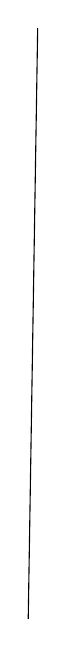
\begin{tikzpicture}[x=1cm,y=1cm]\draw (0,0)--(0.12,7.5);\end{tikzpicture}}}
\margin{the case of characteristic zero is settled in the affirmative by means of the logarithm function --- setting
\[
X+\frac{X^2}{2!}+\cdots+\frac{X^{n-1}}{(n-1)!}=Y,
\]
we shall have
\[
\exp X=1+Y,\quad\text{hence}
\]
\[
X=\log(1+Y)=Y-\frac{Y^2}{2}+\frac{Y^3}{3}\ldots
\]
Works over any base ring of characteristic zero\ldots}
\margin{$\unsure{b|0}$}
i.e. It would have to be that in the case of characteristic 0, it is $\varphi_U$ itself that can already extend to all of $S$. The first doubtful case in this regard seems to me $\unsure{n|m}=5$
\[
(20)\qquad\left\{\begin{array}{l}
\deleted{\unsure{X^5=0}}\quad\inserted{X\in M_5(\unsure{A|K}),\ X^5=0}\\
\displaystyle\frac{X^2}{2}\pm\frac{X^3}{3!}+\frac{X^4}{\deleted{\unsure{2}}4!}\in M_5(A)\\[3pt]
\overset{?}{\Longrightarrow}\quad\deleted{\unsure{X^2,X^3,X^4}}\quad X\in M_5(A)
\end{array}\right.
\]

On the other hand, in the case considered \unsure{a little earlier} ($n=4$, residual characteristic 2 --- the only one that causes difficulties) it is clear that it suffices to take for $d$ a sufficiently large power of 2.

This remark applies to the mixed characteristic cases. We should indeed have this

\uline{Corollary to the lemma} \unsure{dubious} : if $S$ is local, of residual characteristic $p>0$, and if $\varphi$ is defined on an open set which contains $S-V(p)$, (i.e. if the complement of $U$ is of characteristic $p\unsure{>|\geq}0$ --- in fact unnecessary of course that $S$ be local) then $\exists q=p^{\unsure{r|n}}$ such that $\varphi^q$ extends.
\margin{12}

% Pied de page imprimé de l'archive.
\begin{center}
\small
12\\
\texttt{https://grothendieck.umontpellier.fr}\\
Université de Montpellier, UMR CNRS 5149, Case courrier 051, Place Eugène Bataillon\\
34095 Montpellier cedex 5 - France
\end{center}

\scanpage{14}
When $G$ is affine, this should be trivial. We are going to try the

\uline{Proposition} \unsure{Let|Let} $S$ be a quasi-compact prescheme, $n$ an integer $\unsure{\geq1|\geq0}$, \deleted{\unsure{prime|prime}} $S_0=V(n)\subset S$ the closed subscheme defined by $n.1_S$ (thus if $x\in S$, we have $x\in S_0$ iff \deleted{\unsure{characteristic $x$ is of}} \deleted{\unsure{characteristic which divides $n$}} \inserted{characteristic $x\mid n$}), \inserted{$U=S\setminus S_0$,} $G$ an affine group scheme \inserted{of \unsure{finite presentation|finite type}} over $S$, and
\[
(21)\qquad\varphi_U:\mathbb G_a|U\longrightarrow G|U
\]
a group homomorphism. \inserted{We assume $U$ schematically dense in $S$.} Then there exists a \inserted{power} integer \deleted{$d>0$} \inserted{$m=n^{\nu}$ of $n$,} \deleted{such that} and a homomorphism of group schemes
\[
\psi_m:\mathbb G_a\longrightarrow G\unsure{;|,}
\]
such that we have
\[
(22)\qquad\psi_m|U=\bigl(\varphi_U^m:\lambda\longmapsto\varphi_U(\unsure{m\lambda})=\varphi_U(\lambda)^m\bigr)
\]
Let us indeed consider the endomorphism
\[
u_m:\mathbb G_a\longrightarrow\mathbb G_a\qquad\lambda\longmapsto m\lambda
\]
Then formula (22) means that we have commutativity
\diagram{\begin{tikzcd}
\mathbb G_{aU}\arrow[r,dash,"(u_m)_U"]\arrow[dr,"\psi_U"']&\mathbb G_{aU}\arrow[d,"\varphi_U"]\\
&G_U
\end{tikzcd}}
and the existence of the $\unsure{\psi_i|\psi_m}$ for large $m$, means that for large $m$ the composite homomorphism
\[
\deleted{\varphi_U\circ u_m}\qquad\varphi_U\circ u_m:\mathbb G_{aU}\unsure{\longrightarrow|\text{---}}G_U
\]
extends to a group homomorphism $\mathbb G_a\longrightarrow G$.
\margin{13}

% Pied de page imprimé de l'archive.
\begin{center}
\small
13\\
\texttt{https://grothendieck.umontpellier.fr}\\
Université de Montpellier, UMR CNRS 5149, Case courrier 051, Place Eugène Bataillon\\
34095 Montpellier cedex 5 - France
\end{center}

\scanpage{15}
\mspage{655}

For reasons of schematic density and \unsure{uniqueness},
it suffices to prove that $\varphi_U$ extends to a
morphism of \deleted{group} schemes -- \inserted{this} extension will
automatically be a homomorphism of group schemes.
\deleted{$A$ \unsure{that of} \illegible{1} $B$}
\inserted{We may assume $S$ \unsure{Affine}, \unsure{let}}
$A$ be \unsure{its} ring, and let $B$ be that of $G$.
So the ring of $U$ will be
\deleted{$A[1/n]\unsure{=}$}
$A_n\overset{\unsure{\mathrm{déf}}}{=}A[1/n]$, that of $G$ will be
$B\otimes_A A_n=B_n$, by hypothesis we have a homomorphism
(corresponding to $\unsure{\varphi_U^*|\varphi_U}$)
\[
(23)\qquad
\diagram{\begin{tikzcd}
B_n \arrow[r,"\varphi"] & A_n[T]
\end{tikzcd}}
\]
whereas the homomorphism \deleted{\unsure{composite}}
\inserted{corresponding} to $\psi_{mU}$ will be the composite of the preceding one
with
\[
(24)\qquad
\diagram{\begin{tikzcd}
A_n[T] \arrow[r,"\unsure{\psi_m^*|u_m^*}"] & A_n[T] \\
T \arrow[r,mapsto] & mT & \text{thus} & T^i \arrow[r,mapsto] & m^iT^i
\end{tikzcd}}
\]
Let \deleted{$\unsure{x}$}
$\inserted{x=}\,a_0+a_1T+\cdots+a_NT^N\in A_n[T]$ \unsure{of which|thus} the
$a_i\in A_n$ we shall therefore have
\[
\psi_m^*(x)=\sum a_i m^iT^i=\sum(a_i n^{\unsure{i\nu}})T^i
\]
thus if $m=n^\nu$ is large enough, we shall have
\[
\deleted{\psi_m^*(x)\unsure{\sim}m^iT^i\in\unsure{A}}
\]
\[
m^i a_i\in A\quad\text{i.e}\quad m^i a_i\in\unsure{A|T^i}[T]
\qquad \forall i\,\uuline{\unsure{\ge|>}1}
\]
thus
\[
\psi_m^*(x)\equiv a_0\pmod{A[T]}
\]
which shows
\[
(25)\qquad \psi_m(x)\in A[T]\ \text{for }m=n^\nu\text{ large}
\quad\Longleftrightarrow\quad a_0\in A
\]
\margin{14}

% Pied de page imprimé de l'archive.
\begin{center}
\small
14\\
\texttt{https://grothendieck.umontpellier.fr}\\
Université de Montpellier, UMR CNRS 5149, Case courrier 051, Place Eugène Bataillon\\
34095 Montpellier cedex 5 - France
\end{center}

\scanpage{16}

Applying this to the images of elements of $B$ which generate $B$ as
an $A$-algebra, we thus have

\uline{Corollary}\quad $S$ \deleted{$\unsure{S_0}$} $n,S_0,U$ being as in
the proposition, and $G$ being an affine scheme of finite type over $S$
(there is no longer any question of a group structure), and
$\varphi_U:\mathbb E^1_U\longrightarrow G_U$ a morphism of schemes,
\deleted{for there to \unsure{exist}}
$g_U\,\deleted{\unsure{=}}\overset{\unsure{\mathrm{déf}}}{=}\varphi_U(0)$,
For there to exist a \deleted{\illegible{1}} power $m=n^\nu$
of $n$ such that $\varphi_U\circ\unsure{\psi_m|u_m}$
\deleted{\unsure{(where}} (where $u_m$ given by (24)) extends
\inserted{to $S$}, it is necessary and sufficient that $g_U$ extend to a section $g$ of $G$
over $S$.

\uline{Remark}\quad the preceding arguments prove
in any case the \unsure{dubious} ``theorem'' on page \unsure{662|652}'
in the case where $S$ is noetherian of dimension 1
(the case of interest to us being the one where the generic point of $S$
is of characteristic 0).

\margin{\uline{Group schemes} \uline{associated with}
\unsure{extensions of} \uline{discrete groups}}

3.\quad Let $\unsure{M_0|M}$ now be a free $\mathbb Z$-module
of finite type; we are going to construct a
pro-\uline{group} scheme over $S$, associated
with the projective system of sub-\deleted{groups}\inserted{$\mathbb Z$}-modules
of finite index in $M$. To carry out the
construction, I am going to work out \deleted{\unsure{thus}} a
\margin{15}

% Pied de page imprimé de l'archive.
\begin{center}
\small
15\\
\texttt{https://grothendieck.umontpellier.fr}\\
Université de Montpellier, UMR CNRS 5149, Case courrier 051, Place Eugène Bataillon\\
34095 Montpellier cedex 5 - France
\end{center}

\scanpage{17}
\mspage{656}

\margin{I am \unsure{complicating} my life over the construction of
$\underline{\mathfrak S}$, it suffices to set
$\underline{\mathfrak S}=
\mathfrak S_{S_0}\times_{M_{S_0}}\underline M_{S_0}$.}

preliminary exercise, relative to a situation
\[
(26)\qquad
\diagram{\begin{tikzcd}
1 \arrow[r] & M \arrow[r] & \mathfrak S \arrow[r] & H \arrow[r] & 1
\end{tikzcd}}
\]
exact sequence of discrete groups, with $M$ commutative --
the case which \unsure{will interest} us later on being the one where $M$ is a
free $\mathbb Z$-module of finite type. In any case $M$ is a
$\mathbb Z$-module, and as such defines a Group over
$\deleted{\unsure{\mathbb Z}}\inserted{\unsure{S_0}}=\operatorname{Spec}\mathbb Z$,
namely
\[
\diagram{\begin{tikzcd}
A \arrow[r,mapsto] & M\otimes_{\mathbb Z}A
\end{tikzcd}}
\]
($A$, commutative $\mathbb Z$-algebra) -- which we shall denote by $\underline M$.
In fact, $\underline M$ is representable, i.e. is a group \uline{scheme}
iff $M$ is free of finite type.
I feel like also defining \deleted{schemes in} Groups over $S_0$
(which will be group schemes if $M$ is)
$\underline{\mathfrak S},\underline H$, and an exact sequence
\[
(27)\qquad
\diagram{\begin{tikzcd}
1 \arrow[r] & \underline M \arrow[r] &
\underline{\mathfrak S} \arrow[r] & \underline H \arrow[r] & 1
\end{tikzcd}}
\]
of Groups over $S_0$, and an isomorphism of exact sequences
\[
(28)\qquad
\diagram{\begin{tikzcd}
1 \arrow[r] & M \arrow[r] \arrow[d,"\unsure{\wr}"] &
\mathfrak S \arrow[r] \arrow[d,"\unsure{\wr}"] &
H \arrow[r] \arrow[d,"\unsure{\wr}"] & 1 \\
1 \arrow[r] & \underline M(\mathbb Z) \arrow[r] &
\underline{\mathfrak S}(\mathbb Z) \arrow[r] &
\underline H(\mathbb Z) \arrow[r] & 1
\end{tikzcd}}
\]
we shall take
\[
(29)\qquad \underline H=H_{S_0}
\qquad\text{constant Group with value }H
\]
and the outermost vertical arrows of (28)
\margin{16}

% Pied de page imprimé de l'archive.
\begin{center}
\small
16\\
\texttt{https://grothendieck.umontpellier.fr}\\
Université de Montpellier, UMR CNRS 5149, Case courrier 051, Place Eugène Bataillon\\
34095 Montpellier cedex 5 - France
\end{center}

\scanpage{18}

\unsure{will be|are} the canonical isomorphisms.

We can think of defining $\underline{\mathfrak S}$ as
a functor \inserted{(covariant)} in $A/\mathbb Z$ or (\unsure{contravariant})
in $S/S_0$, by
\[
(30)\qquad
\underline{\mathfrak S}(A)=
\mathfrak S\wedge_M
\underbrace{M(A)}_{\deleted{\unsure{A\otimes_{\mathbb Z}}}\inserted{M\otimes_{\mathbb Z}A}}
\]
\deleted{\unsure{As we have}}.
$\underline{\mathfrak S}(A)$ thus being defined as the extension of
$H$ by $M(A)$ \unsure{deduced} from the extension $\mathfrak S$
of $H$ by $M$ by the homomorphism
\[
(31)\qquad
\diagram{\begin{tikzcd}
M \arrow[r] & M\otimes_{\mathbb Z}A
\end{tikzcd}},
\]
which we consider as a homomorphism of $H$-$\mathbb Z$-modules,
by letting $H$ operate on $M\otimes_{\mathbb Z}A$ via its operation on $M$.

The small difficulty is that the \unsure{group|groups}-functor
thus defined by (30) is not itself representable --
it gives the correct expression for $\underline{\mathfrak S}(A)$ only if
$\operatorname{Spec}A$ is connected -- it corresponds to the subfunctor of
\[
\begin{array}{c}
\inserted{\unsure{\sim}}\\[2pt]
\diagram{\begin{tikzcd}
S \arrow[r,mapsto] &
\unsure{:}\underline{\mathfrak S}(A)=
\deleted{\unsure{\operatorname{Spec}|\underline{\mathfrak S}}}
\underline{\mathfrak S}(S)
\end{tikzcd}}
\qquad (S=\operatorname{Spec}A)
\end{array}
\]
consisting of the \deleted{points such that the}
\inserted{$S\longrightarrow\underline{\mathfrak S}$}
such that the composite
\[
(32)\qquad
\diagram{\begin{tikzcd}
S \arrow[r] & \underline H_S
\end{tikzcd}}
\]
(which corresponds to a \uuline{locally} \uline{\unsure{constant|constant}}
function on $S$ with values in $H$) is
\inserted{(\unsure{entirely})} constant.
\margin{17}

% Pied de page imprimé de l'archive.
\begin{center}
\small
17\\
\texttt{https://grothendieck.umontpellier.fr}\\
Université de Montpellier, UMR CNRS 5149, Case courrier 051, Place Eugène Bataillon\\
34095 Montpellier cedex 5 - France
\end{center}

\scanpage{19}
\mspage{657}

The correct expression will be obtained by starting from the \inserted{\illegible{1}} ``incorrect'' functor
\[
\diagram{\begin{tikzcd}
{[\underline{\mathfrak S}]: A} \arrow[r,mapsto] &
\mathfrak S\wedge_M(M\otimes_{\mathbb Z}A)
\end{tikzcd}}
\]
\unsure{or} better, from the \unsure{contravariant functor|contrafunctor}
\[
\diagram{\begin{tikzcd}
S \arrow[r,mapsto] &
\mathfrak S\wedge_M
\Gamma(S,M\otimes_{\mathbb Z}\underline{\unsure{\mathcal O|O}}_S)
\end{tikzcd}},
\]
and taking the associated Zariski sheaf -- in fact we shall have. $=$
\[
(33)\qquad
\underline{\mathfrak S}(S)=
\underset{\mathcal U=(U_i)_{i\in\unsure{S|I}}}{\varinjlim}
\prod_{i\in I}[\mathfrak S](U_i)
\]
\[
\begin{array}{l}
(U_i)_{i\in I}\ \text{a partition}\\
\text{of }S\text{ into }\unsure{\text{schemes}}\\
\unsure{\text{open}}\qquad S\simeq\coprod U_i
\end{array}
\]

Here is another way of presenting the construction of
$\underline{\mathfrak S}$, using the general construction
of §49 -- in the sheaf-theoretic context. We have a system
\[
(34)\qquad
\underbrace{\underline M}_{\text{Group over }S_0},
\quad
\underbrace{\mathfrak S_{S_0}
\overset{\cdot}{\supset}\unsure{M}_{S_0}}_{
\substack{\text{Groups (constant)}\\
\text{over }S_0,\ M_{S_0}\\
\text{normal}}},
\quad
\mathrm{Op.}^{\unsure{\Theta|\theta}}\text{ of }
\mathfrak S_{S_0}\text{ on }\underline M,
\]
\[
\diagram{\begin{tikzcd}
\text{homomorphism }\varphi:
\deleted{\unsure{\mathfrak S}}\inserted{M}_{S_0}
\arrow[r] & \underline M
\end{tikzcd}}
\]
(where the operation of $\mathfrak S_{S_0}$ on $\underline M$,
which \unsure{amounts} to an operation of $\mathfrak S$ on $\underline M$,
is the one deduced from the operation of $\mathfrak S$ on $M$,
by \unsure{functoriality})
these data \unsure{satisfying} the compatibility conditions a) b)
of loc. cit. By the construction \unsure{of|of} loc. cit., we construct
\margin{18}

% Pied de page imprimé de l'archive.
\begin{center}
\small
18\\
\texttt{https://grothendieck.umontpellier.fr}\\
Université de Montpellier, UMR CNRS 5149, Case courrier 051, Place Eugène Bataillon\\
34095 Montpellier cedex 5 - France
\end{center}
